%Copyright 2019 Christopher M. Jermaine (cmj4@rice.edu) and Risa B. Myers (rbm2@rice.edu)
%
%Licensed under the Apache License, Version 2.0 (the "License");
%you may not use this file except in compliance with the License.
%You may obtain a copy of the License at
%
%    https://www.apache.org/licenses/LICENSE-2.0
%
%Unless required by applicable law or agreed to in writing, software
%distributed under the License is distributed on an "AS IS" BASIS,
%WITHOUT WARRANTIES OR CONDITIONS OF ANY KIND, either express or implied.
%See the License for the specific language governing permissions and
%limitations under the License.
%===============================================================
\documentclass[aspectratio=169]{beamer}
\mode<presentation>
{
\usetheme[noshadow, minimal,numbers,riceb,nonav]{Rice}
\usefonttheme[onlymath]{serif}
\setbeamercovered{transparent}
}
\useinnertheme{rectangles}

\usepackage[english]{babel}

\usepackage{mathptmx}
\usepackage{helvet}
\usepackage{courier}
\usepackage[T1]{fontenc}
\usepackage{trajan}
\usepackage{ textcomp }
\usepackage{listings}

\newenvironment{noindentitemize}
{ \begin{itemize}
 \setlength{\itemsep}{1.5ex}
  \setlength{\parsep}{0pt}   
  \setlength{\parskip}{0pt}
 \addtolength{\leftskip}{-2em}
 }
{ \end{itemize} }

\newenvironment{noindentitemize2}
{ \begin{itemize}
  \setlength{\itemsep}{0ex}
  \setlength{\parskip}{0pt}
  \setlength{\parsep}{0pt}   
  \addtolength{\leftskip}{-2em}  }
{ \end{itemize} }



\lstnewenvironment{SQL}
  {\lstset{
        aboveskip=5pt,
        belowskip=5pt,
        escapechar=!,
        mathescape=true,
        upquote=true,
        language=SQL,
        basicstyle=\linespread{0.94}\ttfamily\footnotesize,
        morekeywords={PRINT, CURSOR, OPEN, FETCH, CLOSE, DECLARE, BEGIN, END, PROCEDURE, FOR, EACH, WITH, PARTITION, 	TEST, WHETHER, PROBABILITY, OUT,LOOP,IF,CONTINUE, HANDLER,CALL, FUNCTION, RETURNS, LANGUAGE,BODY,RETURN, REPLACE,plpgsql,
        RAISE, NOTICE,
        REPLACE, ROW, BEFORE, EXIT, TEXT, REFCURSOR, QUOTE_LITERAL, DELIMITER,CONCAT,FOUND,LEAVE },
        deletekeywords={VALUE, PRIOR},
        showstringspaces=true}
        \vspace{0pt}%
        \noindent\minipage{0.65\textwidth}}
  {\endminipage\vspace{0pt}}
  
  
\lstnewenvironment{SQLtiny}
  {\lstset{
        aboveskip=5pt,
        belowskip=5pt,
        escapechar=!,
        mathescape=true,
        upquote=true,
        language=SQL,
        basicstyle=\linespread{0.94}\ttfamily\tiny,
        morekeywords={PRINT, CURSOR, OPEN, FETCH, CLOSE, DECLARE, BEGIN, END, PROCEDURE, FOR, EACH, WITH, PARTITION, 	TEST, WHETHER, PROBABILITY, OUT,LOOP,IF,CONTINUE, HANDLER,CALL, FUNCTION, RETURNS, LANGUAGE,BODY,RETURN, REPLACE,plpgsql,
        RAISE, NOTICE,
        REPLACE, ROW, BEFORE, EXIT, TEXT, REFCURSOR, QUOTE_LITERAL, DELIMITER,CONCAT,FOUND,LEAVE },
       deletekeywords={VALUE, PRIOR},
        showstringspaces=true}
        \vspace{0pt}%
        \noindent\minipage{0.47\textwidth}}
  {\endminipage\vspace{0pt}}

%===============================================================%

\title[]
{Tools \& Models for Data Science}

\subtitle{Big Data Part One: An Introduction to MapReduce}

\author[]{Chris Jermaine \& Risa Myers}
\institute
{
  Rice University 
}

\date[]{}

\subject{Beamer}


\begin{document}

\begin{frame}
 \titlepage
\end{frame}


%***********************************************************
\begin{frame}{15 Years Ago...}

\begin{itemize}
\item Say you had a big data set, wanted platform to analyze it
\item What is ``big''?
	\begin{itemize}
	\item Too large to fit in RAM of an expensive server machine
	\item ``Big Data'' termed appeared in late 90's % credited to John R. Mashey , Chief Scientist SGI 
	\end{itemize}
\item Is 5GB in 2002, a couple of terabytes in 2018
\item You might spend \$20 - 30K on a server
\end{itemize}
\end{frame}
%***********************************************************
\begin{frame}{The 5 V's of ``Big'' Data}
\begin{columns}[c]
\column{.3\textwidth} % Left column and width
\begin{enumerate}
\item Volume % at rest quantity 
\item Variety  % different forms
\item Velocity % speed - in motion
\item Veracity % in doubt
\item Value % TCO (total cost of ownership) & ROI
\end{enumerate}
\column{.6\textwidth} % Right column and width
    	{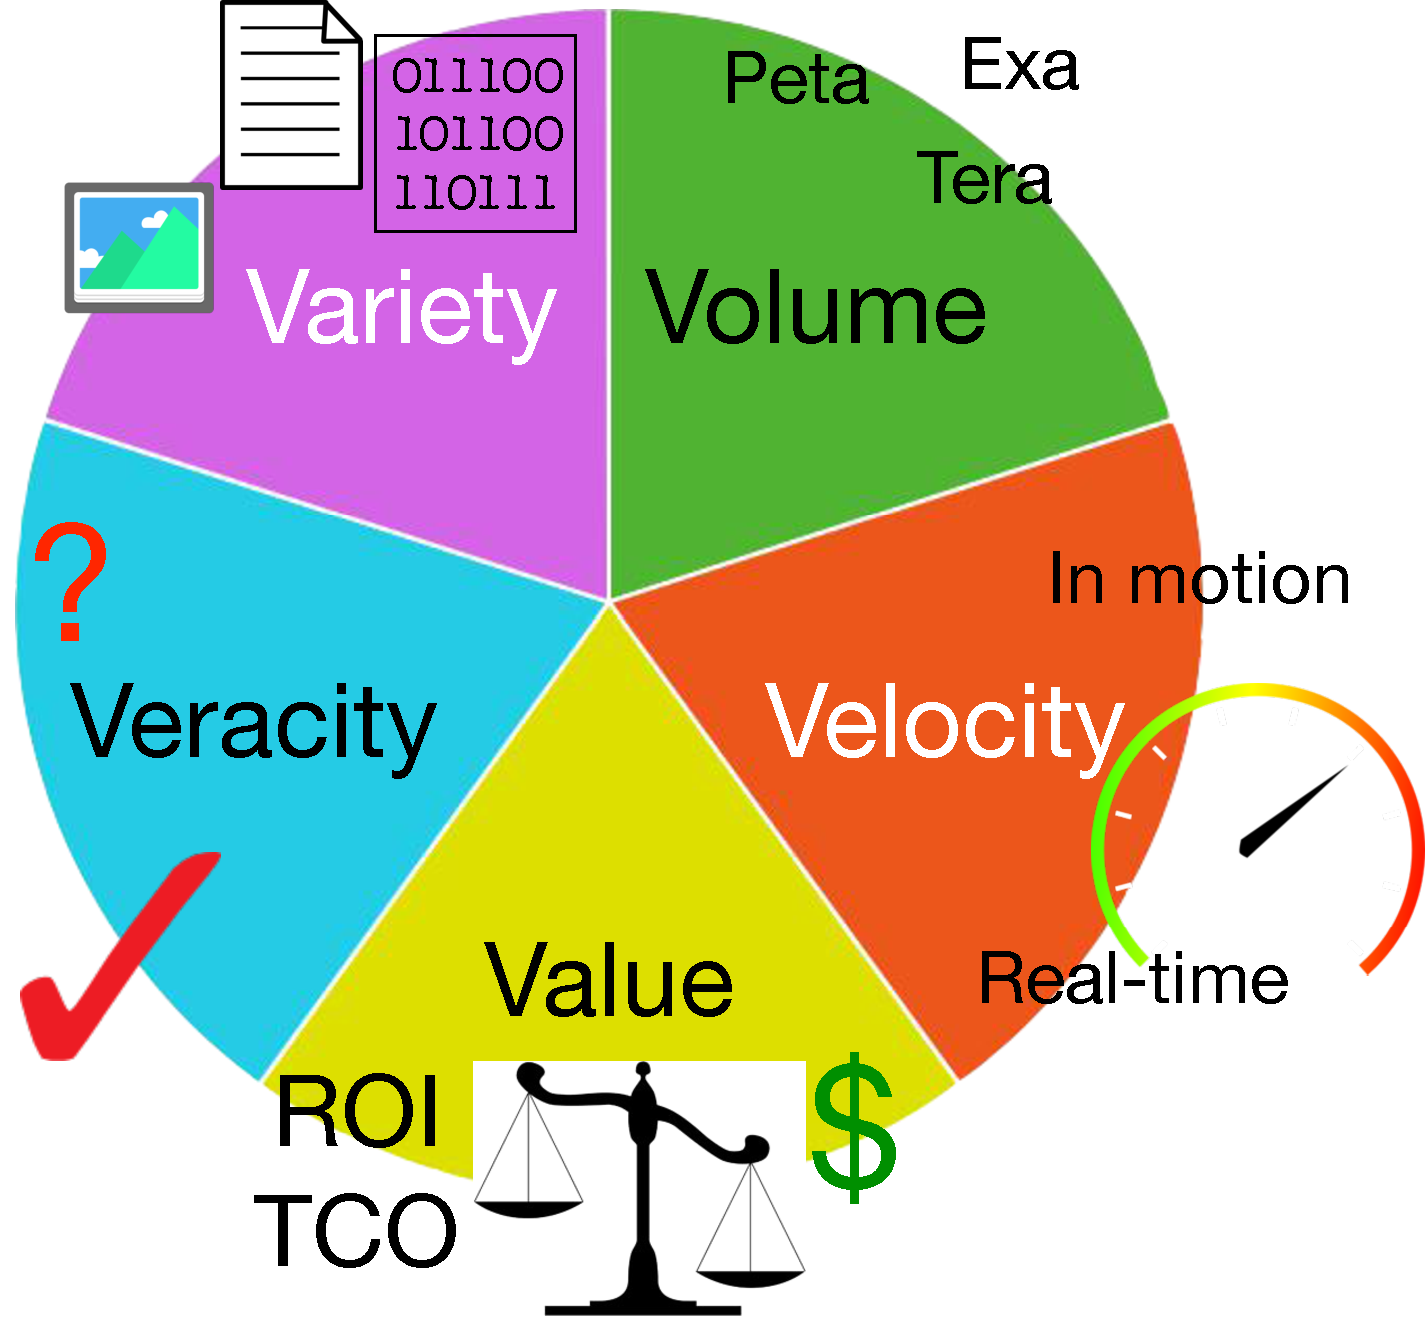
\includegraphics[width=1\textwidth]{./lectBigData/5vsV2.pdf}} \\
\end{columns}
\end{frame}

%***********************************************************
\begin{frame}{7 V's}

\begin{enumerate}
\item Volume % at rest quantity 
\item Variety  % different forms
\item Velocity % speed - in motion
\item Veracity % in doubt
\item Value % TCO (total cost of ownership) & ROI
\item {\textcolor{red}{Variability}} % changes in quality over time
\item {\textcolor{red}{Visualization}} 
\end{enumerate}
\end{frame}

%***********************************************************
\begin{frame}{How to Analyze a ``Big'' Dataset}

\begin{itemize}
\item You might write your own sofware
\item Costly, time consuming
        \begin{itemize}
        \item A \$10M software feature might eat up most of the IT budget for a single firm
        \end{itemize}
\item Requires expertise not always found in house
\item Risky: high potential for failure
\end{itemize}
\end{frame}
%***********************************************************
\begin{frame}{Or, You Might Buy a DB System}

\begin{itemize}
\item Costs a LOT of money
\item Performance often unpredictable, or just flat out poor
\item Software can be insanely complicated to use correctly
\item Software stack too big/deep, not possible to unbundle
	\begin{itemize}
	\item If you are doing analysis, ACID not important
	\item And yet, you pay for it (money, complexity, performance)
	\end{itemize}
\item Difficult to put un- or semi-structured data into an SQL DB
\end{itemize}

\end{frame}
%***********************************************************
\begin{frame}{Plus, Many People Just Don't Like SQL}

\begin{itemize}
\item People uncomfortable with declarative programming
        \begin{itemize}
        \item We love it!
	\item But users don't really know what's happening under the hood
	\item Makes many programmers uncomfortable
        \end{itemize}
\item Also, not easy/natural to specify important computations
        \begin{itemize}
        \item Especially data mining and machine learning
	\item Not to mention High Performance Computing-style computations  (Analytics)
        \end{itemize}
\end{itemize}
\end{frame}
%***********************************************************
\begin{frame}{By Early-Mid 2000's...}

\begin{itemize}
\item The Internet companies (Google, Yahoo, etc.)...
        \begin{itemize}
        \item ...had some of the largest databases in the world
        \item But they never used classical SQL databases for webscale
        \end{itemize}
\item How'd they do it?
        \begin{itemize}
        \item Many ways...
	\item But paradigm with most widespread impact was MapReduce
	\item First described in a 2004 academic paper, appeared in Operating Systems Design and Implementation (OSDI)
	% top tier conference
	\item  ``MapReduce: Simplified Data Processing on Large Clusters''
        \end{itemize}
\end{itemize}
\end{frame}
%***********************************************************
\begin{frame}{Stage is set for a New Paradigm}

\begin{itemize}
\item Existing approaches don't work
\begin{itemize}
\item Custom software is too expensive
\item RDBMSs are too rigid
\end{itemize}
\item Data volume has exploded
\item Commodity hardware has become cheap
\item Cost is proportional to workload
\item Welcome MapReduce!
\end{itemize}
\end{frame}
%%***********************************************************
%\begin{frame}{Why Commodity Hardware?}
%
%\begin{itemize}
%\item Hard drives and computers fail all the time
%\item Some estimates are 5\% of hard drives fail in the first year of operation %https://www.extremetech.com/computing/170748-how-long-do-hard-drives-actually-live-for
%\item When you have lots of data and lots of computers, this rapidly becomes a lot of failures
%\item So, you accept it and build in redundancy and recovery
%\item Highly scalable
%\end{itemize}
%\end{frame}
%***********************************************************
\begin{frame}{What Is MapReduce?}

\begin{itemize}
\item A simple data processing paradigm
\item Leverages a cluster of commodity machines
\begin{itemize}
\item For distributed processing
\item For fault tolerance
\item Requires a distributed file system % this is the persisting contribution
\item See ``The Google File System'' by Ghemawat, et al. 2003
\end{itemize}
\item Well suited to calculations that can be computed in independent chunks
\end{itemize}
\end{frame}

%***********************************************************
\begin{frame}[fragile]{What Is Novel about MapReduce?}

\begin{itemize}
\item  Novelty is in scalability and fault tolerance
\item The functional model already existed
\item Consider the map and reduce functions in Python
\item Map:

%\texttt{map(<function>, <inputs>)}

\texttt{items = [ 1, 2, 3, 4, 5 ]}

\texttt{mod2 = list(map(lambda x: x \% 2, items))}

\hspace{4.75em}\texttt{[ 1, 0, 1, 0, 1 ]}

\item Reduce:

\texttt{from functools imoport reduce}

\texttt{mySum = reduce((lambda x,y: x + y), items)}

\texttt{15}
\end{itemize}
\end{frame}


%***********************************************************
\begin{frame}{MapReduce}

\begin{itemize}
\item To process a data set:
        \begin{itemize}
        \item You have two pieces of user-supplied code
	\item A Map code
	\item And a Reduce code
        \end{itemize}
\end{itemize}
\end{frame}
%***********************************************************
\begin{frame}{MapReduce}

\begin{itemize}
\item These are run in a huge shared-nothing compute cluster
        \item Using three data processing phases
        \begin{enumerate}
        \item A Map phase
        \item A Shuffle phase
        \item And a Reduce phase
        \end{enumerate}
\end{itemize}

\end{frame}
%***********************************************************
\begin{frame}{First: What Is Shared-Nothing?}

\begin{columns}[c]
\column{.65\textwidth} % Left column and width
\begin{itemize}
\item Store/analyze data on a large number of commodity machines
        \begin{itemize}
	\item Local, non-shared storage attached to each of them
	\item Only link is via a LAN
        \item Shared nothing refers to no sharing of RAM, storage
	\item Note: Network Attached Storage (NAS) is common now, ``pure'' shared-nothing rarer 
        \end{itemize}
\end{itemize}
\column{.35\textwidth} % Right column and width
    	{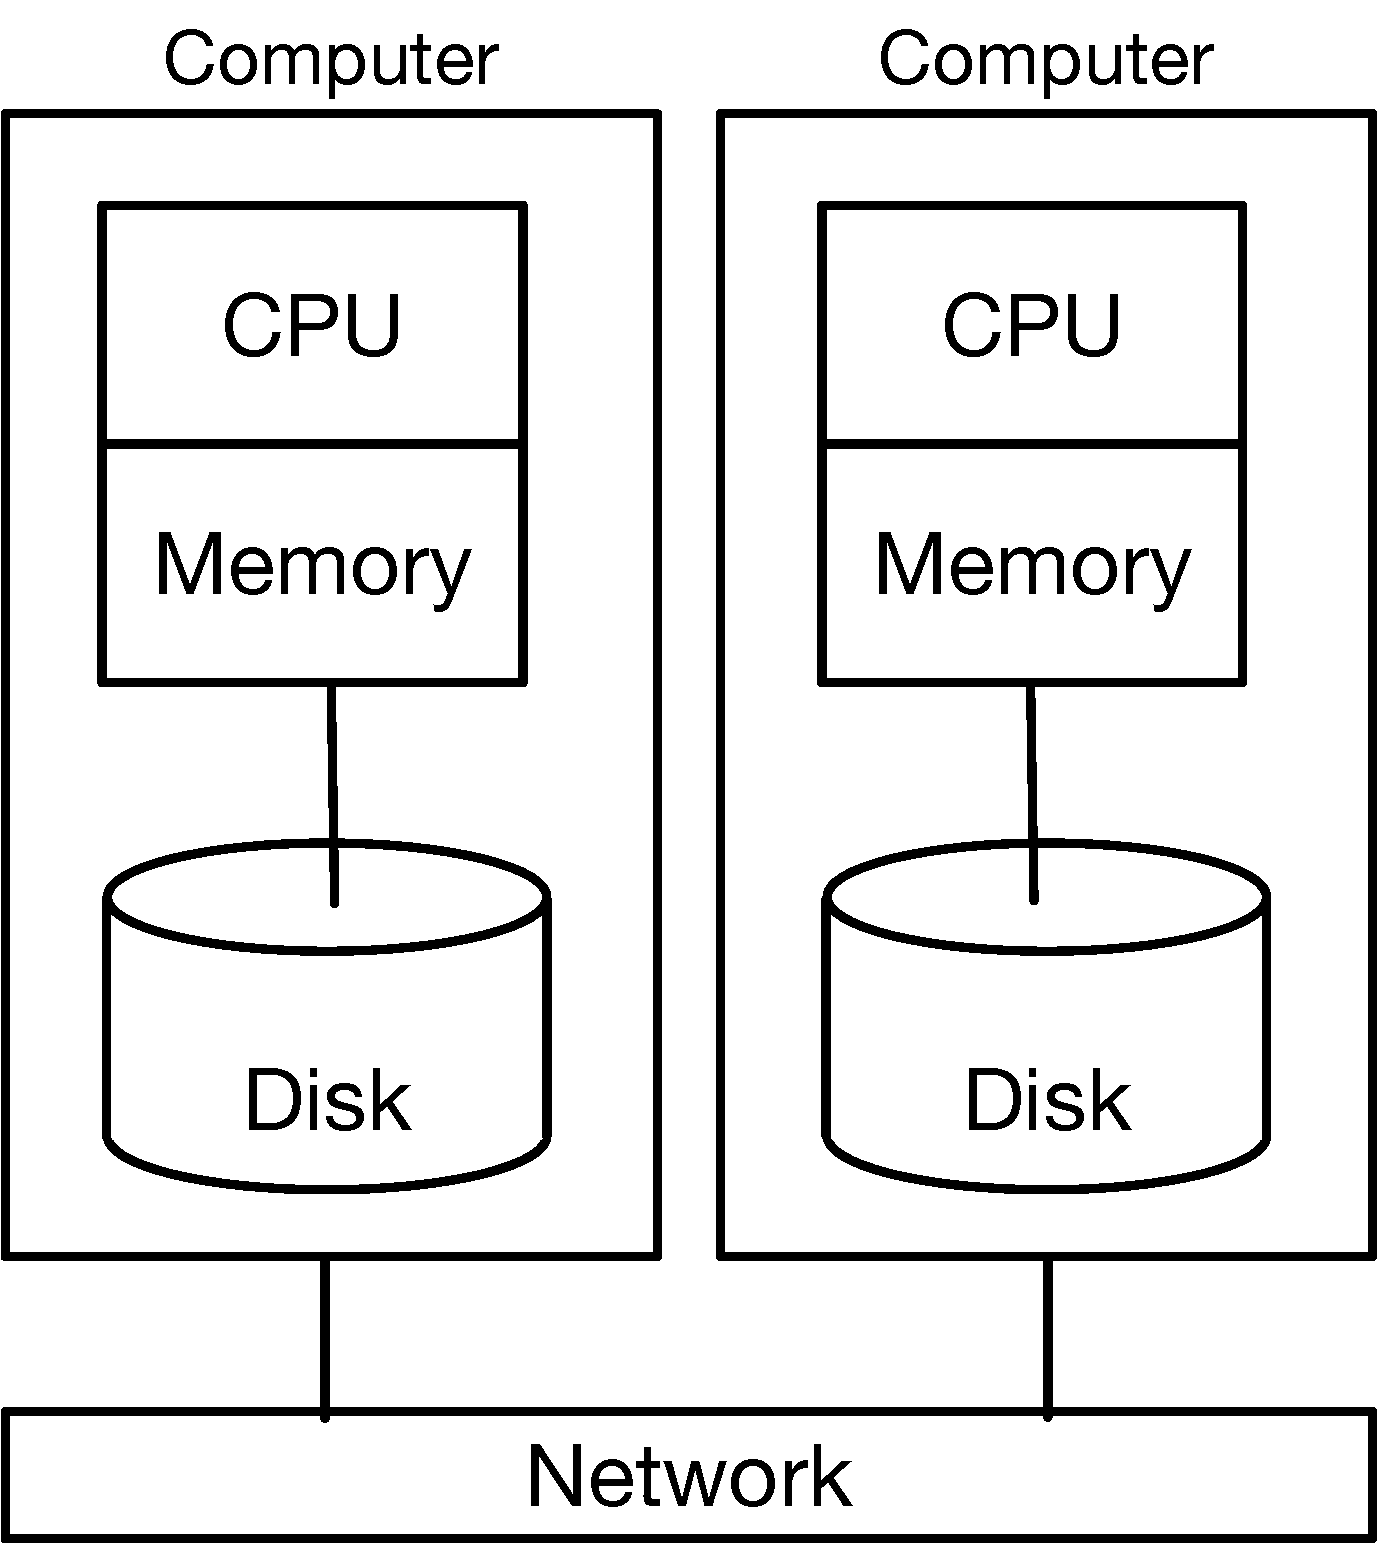
\includegraphics[width=1\textwidth]{./lectBigData/sharedNothing.pdf}} \\
\end{columns}
\end{frame}
%***********************************************************
\begin{frame}{Benefits of Shared-Nothing}

\begin{itemize}
        \item Inexpensive, built out of commodity components
	\item Compute resources scales nearly linearly with money
        \item Contrast to shared RAM machine with uniform memory access
        \item Easier to program than Shared Memory systems
\end{itemize}
\end{frame}
%***********************************************************
\begin{frame}{MapReduce: The Map Phase}

\begin{columns}[c]
\column{.65\textwidth} % Left column and width
\begin{itemize}
\item Input data are stored in a huge file
        \begin{itemize}
        \item Contains a simple list of pairs of type $(key1,value1)$
        \end{itemize}
\item Have a UDF (user defined function) of the form $Map(key1,value1)$
        \begin{itemize}
        \item Outputs a list of pairs of the form ($key2, value2)$
        \end{itemize}
\item During the Map phase of the MapReduce computation
        \begin{itemize}
        \item The $Map$ function is called for every record in the input 
	\item Instances of $Map$ run in parallel all over the cluster
        \end{itemize}
\end{itemize}
\column{.35\textwidth} % Right column and width
Task: Compute the number of occurrences of each token
    	{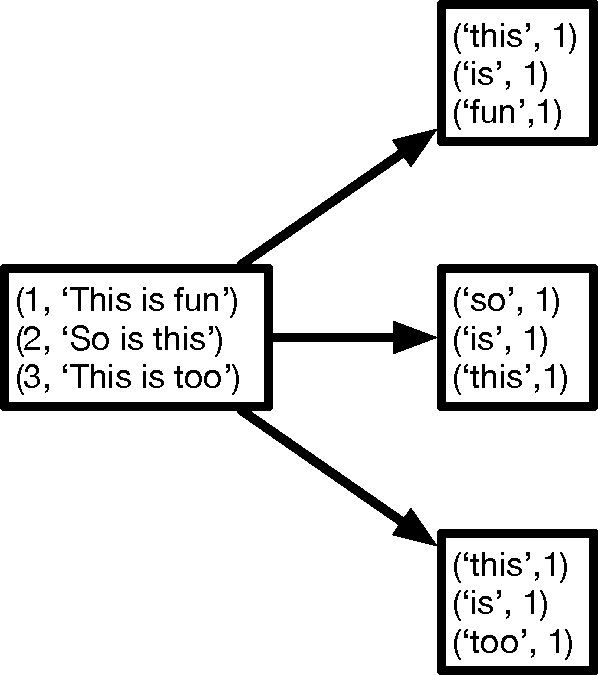
\includegraphics[width=1\textwidth]{./lectBigData/map.pdf}} \\
\end{columns}
% UDF may ignore the key
\end{frame}

%***********************************************************
\begin{frame}{Example: Word Count}

\begin{itemize}
\item Large text corpus
\item Want to count number of occurences of each word
\item Ex output: (`The', 1832321), (`An', 1732432), etc.
\item To power the Map phase, MapReduce software automatically:
        \begin{itemize}
\item  Breaks the corpus into large number of $(lineNo, text)$ pairs
\item Distributes the Map UDF
\item Distributes the fragments
\item Ensures that the UDF is run on all the fragments
        \end{itemize}
\end{itemize}

\end{frame}
%***********************************************************
\begin{frame}{MapReduce: The Shuffle Phase}

\begin{columns}[c]
\column{.65\textwidth} % Left column and width
\begin{itemize}
\item Accepts all of the $(key2, value2)$ pairs from the Map phase
        \begin{itemize}
        \item And it groups them together
        \end{itemize}
\item After grouping, all of the pairs
        \begin{itemize}
        \item From all over the cluster having the same $key2$ value
	\item Are merged into a single $(key2, itemize \langle value2 \rangle)$ pair
        \end{itemize}
\item Called a ``Shuffle''...
        \begin{itemize}
        \item Because this is where a potential all-to-all data transfer happens
        \item Can be expensive
        \item Often implemented using a hash function to map keys to nodes
transfer happens
        \end{itemize}
\end{itemize}
\column{.3\textwidth} % Right column and width
    	{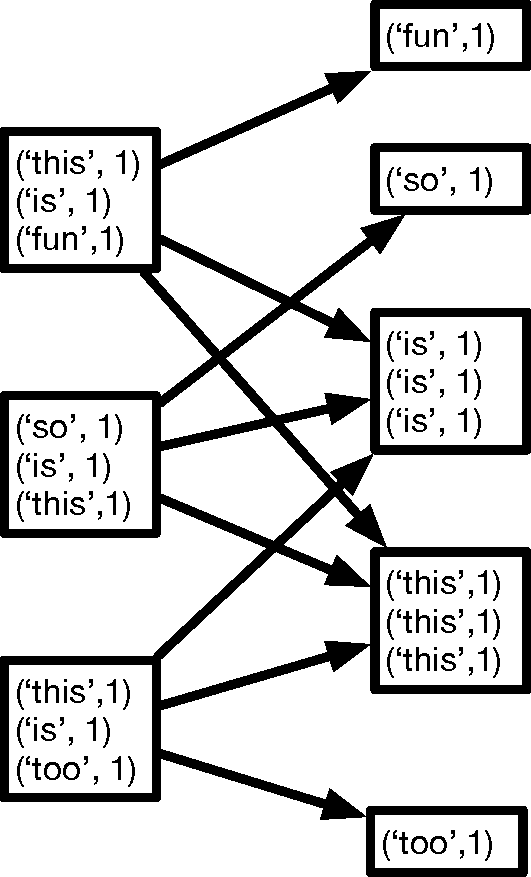
\includegraphics[width=1\textwidth]{./lectBigData/shuffle.pdf}} \\
\end{columns}

\end{frame}
%***********************************************************
\begin{frame}{MapReduce: The Reduce Phase}

\begin{columns}[c]
\column{.6\textwidth} % Left column and width
\begin{itemize}
\item Have a user-supplied function of the form
        \begin{itemize}
        \item $Reduce (key2, itemize \langle value2 \rangle)$
	\item Outputs a list of $value3$ objects
        \end{itemize}
\item In the Reduce phase of the MapReduce computation
        \begin{itemize}
        \item $Reduce$ function is called for every $key2$ value output by the Shuffle
        \item Instances of $Reduce$ run in parallel all over the compute cluster
	\item The output of all of those instances is collected
	\item Put in a (potentially) huge output file
        \end{itemize}
\end{itemize}
\column{.4\textwidth} % Right column and width
    	{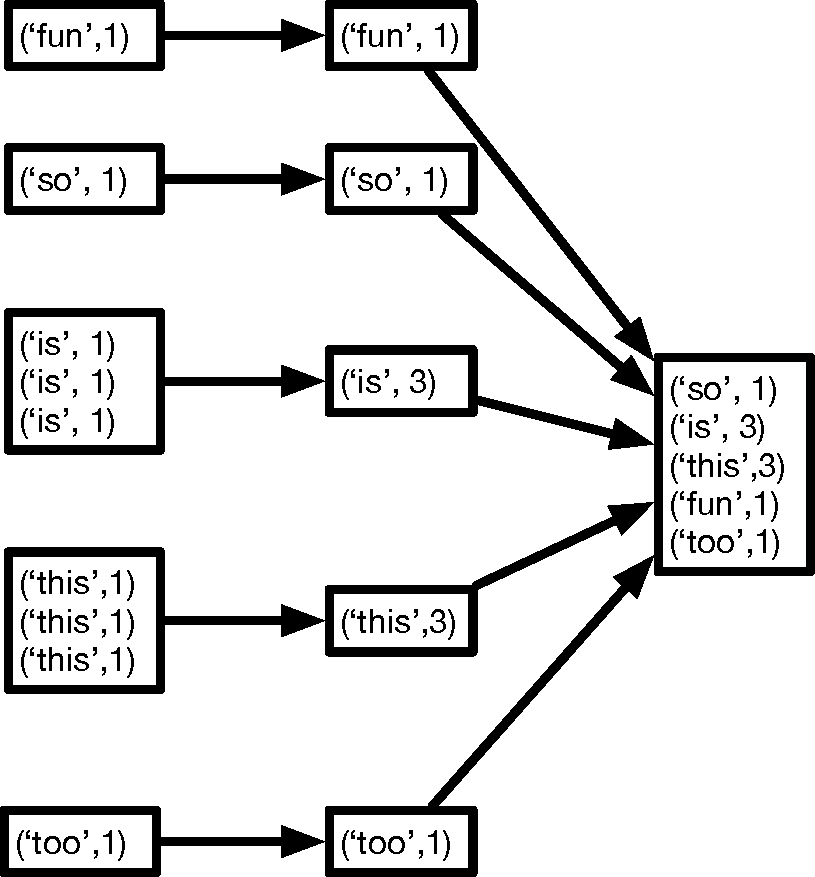
\includegraphics[width=1\textwidth]{./lectBigData/reduce.pdf}} \\
\end{columns}
\end{frame}

%***********************************************************
\begin{frame}{MapReduce: All Phases}

\begin{center}
    	{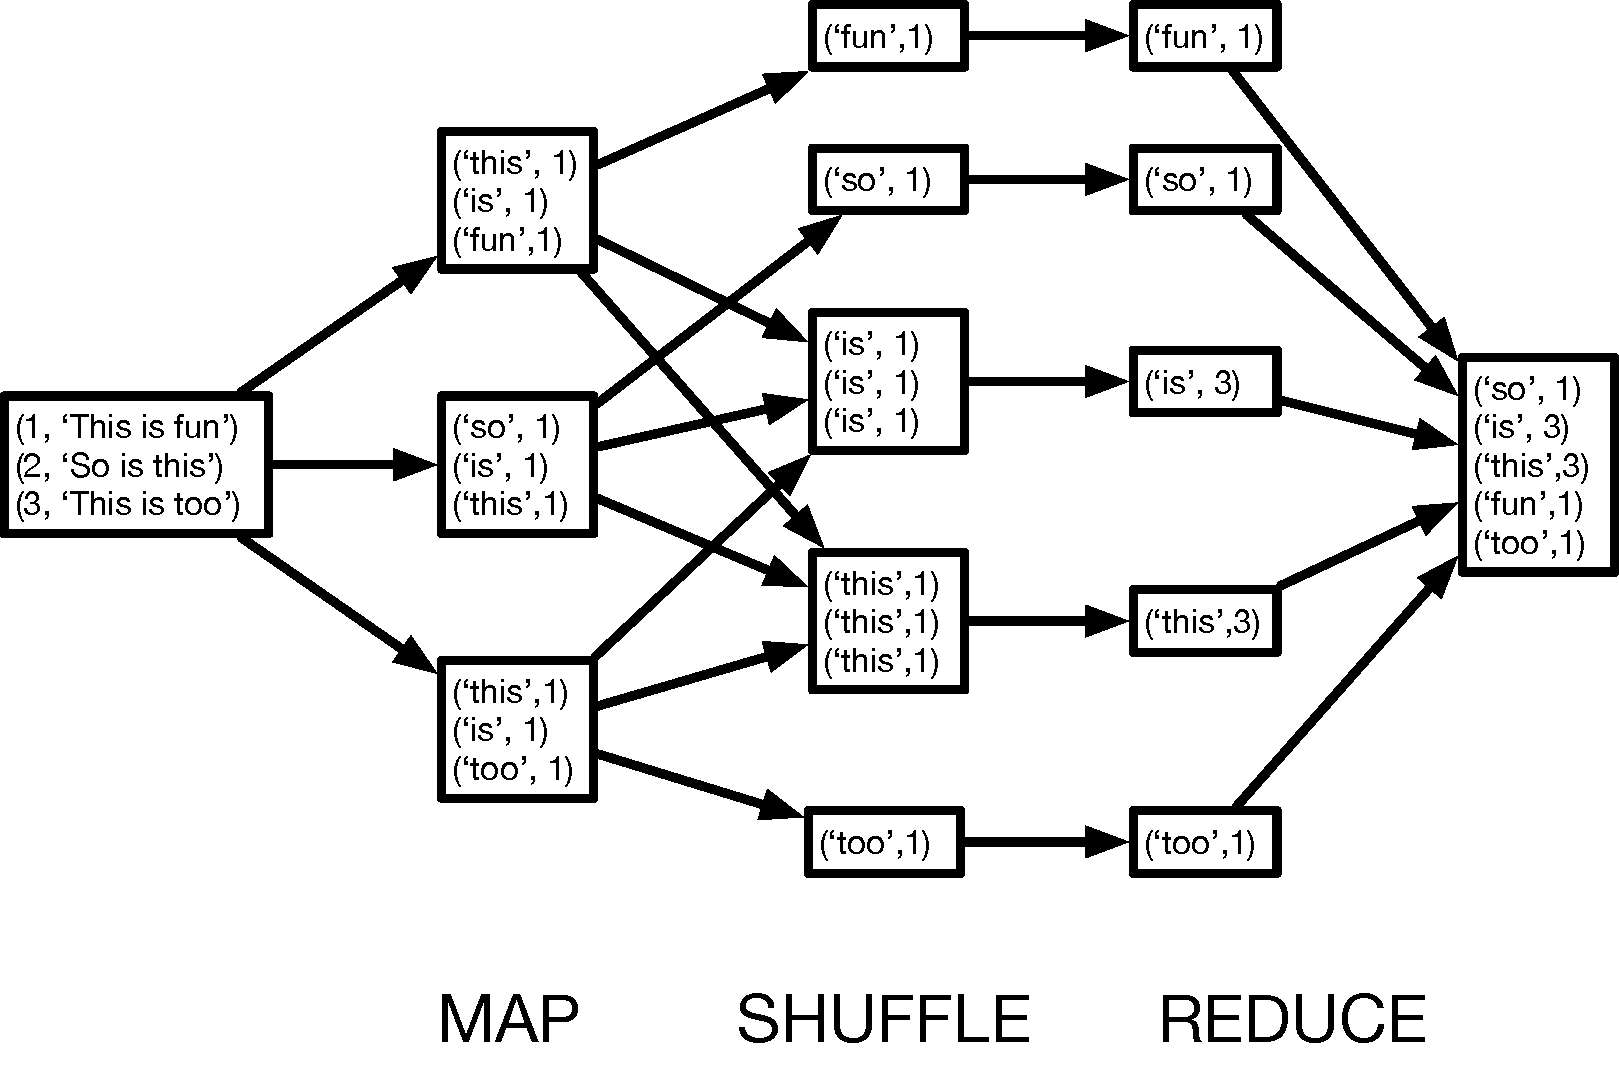
\includegraphics[width=.8\textwidth]{./lectBigData/MRphases.pdf}} 
\end{center}

	
\end{frame}
%***********************************************************
\begin{frame}{MapReduce is a Compute Paradigm}

\begin{itemize}
\item It is not a data storage paradigm
        \begin{itemize}
	\item But must read/write data from some storage
system
        \end{itemize}
\item So MapReduce is strongly linked with the idea of a distributed file system (DFS)
        \begin{itemize}
        \item Allows data to be stored/accessed
across machines in a network
        \item Abstracts away differences between local and remote data
        \item Uses the same API to read/write data
        \item Regardless of network location
        \end{itemize}
\end{itemize}
\end{frame}
%***********************************************************
\begin{frame}{Distributed File Systems for MR}

\begin{itemize}
\item DFSs have been around for a long time
        \begin{itemize}
        \item First widely used DFS was Sun's NFS, first introduced in 1985
        \item Intended to be allow file access across networks as if file was local
        \end{itemize}
\item Unlike classical DFS...
        \begin{itemize}
	\item MapReduce DFS sits on top of each machine's OS
        \item Lives in ``user space''
        \item The OS is not aware of the DFS
        \item You can't mount it anywhere
        \end{itemize}
\item Why on top of, not in the OS?
	\begin{itemize}
	\item Heterogeneity no problem (each machine can run a different OS)
	\item Easily portable (JVM)
	\end{itemize}
\item Even as MapReduce becomes less popular, MR DFS lives on!
\end{itemize}
\end{frame}
%***********************************************************
\begin{frame}{MapReduce vs. HPC}

\begin{itemize}
\item MapReduce pros
	\begin{itemize}
	\item MUCH lower programmer burden than HPC
	\item No synchronization, all parallelism is implicit
	\item Data and task placement automatic
	\item Built-in fault tolerance
	\item Works with (almost!) arbitrarily-sized data
	\item Out-of-core execution is no problem
	\end{itemize}
\end{itemize}
\end{frame}
%***********************************************************
\begin{frame}{MapReduce vs. HPC}

\begin{itemize}
\item MapReduce cons
        \begin{itemize}
        \item Standard softwares are JVM-based
        \item Not suitable for communication-heavy tasks...
	\item ...only communication is via the shuffle
        \item Assumes BIG data... always reads/writes data from DFS
        \end{itemize}
\end{itemize}
\end{frame}
%***********************************************************

\begin{frame}{Wrap up}
\begin{itemize}
	\item[?] How can we use what we learned today?
	\vspace{2em}
	\item[?] What do we know now that we didn't know before?
\end{itemize}


\end{frame}



\end{document}
